%\textsl{}%!TEX TS-options = --shell-escape
%!TEX TS-program = pdflatex
\documentclass[%
   10pt,              % Schriftgroesse
   ngerman,           % wird an andere Pakete weitergereicht
   a4paper,           % Seitengroesse
   DIV11,             % Textbereichsgroesse (siehe Koma Skript Dokumentation !)
]{scrartcl}%     Klassen: scrartcl, scrreprt, scrbook, article
% -------------------------------------------------------------------------

\usepackage[utf8]{inputenc} % Font Encoding, benoetigt fuer Umlaute
\usepackage[english]{babel}   % \textsl{}Spracheinstellung

\usepackage[T1]{fontenc} % T1 Schrift Encoding
\usepackage{textcomp}    % Zusatzliche Symbole (Text Companion font extension)
\usepackage{lmodern,dsfont}     % Latin Modern Schrift
\usepackage{dsfont}
%\usepackage{wasysym}
\usepackage{ulem}
\usepackage{graphicx}
\usepackage{eurosym}
%\usepackage{txfonts}
\usepackage{stmaryrd}
\usepackage{amsfonts}
\usepackage{amsmath}
\usepackage{hyperref}
\usepackage{tikz}
\usepackage{multirow}
\usepackage{listings}
\usepackage{etextools}
\usepackage{ifthen}
%\usepackage{TikZ} %phylogenetischer Baum
%\usetikzlibrary{calc, shapes, backgrounds} %für die Phylogenetische bäume
%\usetikzlibrary{automata,arrows}
\usepackage{subfigure} 


% Definition des Headers
\usepackage{geometry}
\geometry{a4paper, top=3cm, left=3cm, right=3cm, bottom=3cm, headsep=0mm, footskip=0mm}
\renewcommand{\baselinestretch}{1.3}\normalsize

\def\header#1#2#3#4#5#6#7{\pagestyle{empty}
\noindent
\begin{minipage}[t]{0.6\textwidth}
\begin{flushleft}
\textbf{#4}\\% Fach
#6\\% Semester
Tutor: #2  % Tutor 
\end{flushleft}
\end{minipage}
\begin{minipage}[t]{0.4\textwidth}
\begin{flushright}
\points{#7}% Punktetabelle
\vspace*{0.2cm}
#5%  Names
\end{flushright}
\end{minipage}

\begin{center}
{\Large\textbf{ Blatt #1}} % Blatt

{(Abgabe am #3)} % Abgabedatum
\end{center}
}

\newenvironment{vartab}[1]
{
    \begin{tabular}{ |c@{} *{#1}{c|} } %\hline
}{
    \end{tabular}
}

\newcommand{\myformat}[1]{& #1}

\newcommand{\entry}[1]{
  \edef\result{\csvloop[\myformat]{#1}}
  \result \\ \hline
}

\newcommand{\numbers}[1]{
  \newcounter{ctra}
\setcounter{ctra}{1}
\whiledo {\value{ctra} < #1}%
{%
  \myformat{\thectra}
  \stepcounter{ctra}%
}
\myformat{\thectra}
}
\newcommand{\emptyLine}[1]{
  \newcounter{ctra1}
\setcounter{ctra}{1}
\whiledo {\value{ctra1} < #1}%
{%
  \myformat{\hspace*{0.5cm}}
  \stepcounter{ctra1}%
}
}

\newcommand{\points}[1]{
\newcounter{colmns}
\setcounter{colmns}{#1}
\stepcounter{colmns}
  \begin{vartab}{\thecolmns}
    \numbers{#1} & $\sum$ (6+2)\\\hline
    \emptyLine{\thecolmns}\\
  \end{vartab}
}

\begin{document}
%\header{Blatt}{Tutor}{Abgabedatum}{Vorlesung}{Bearbeiter}{Semester}{Anzahl Aufgaben}
\header{8}{Alexander Seitz}{14. December 2015}{Bioinformatics I}{\\Jonas Ditz \\\& Benjamin Schroeder}{WS 15/16}{2}

\section*{Theoretical Assignment - \textit{Suffix tree construction and application}}

\subsection*{a - \textit{Suffix tree construction}}
\subsubsection*{i}
If one uses the naive approach to construct the suffix tree of ``CTAGTAGCAG'', the result would look 
like Figure \ref{fig:naiveImpl}.

\begin{figure}[ht]
 \centering
 \subfigure[step 1]{
  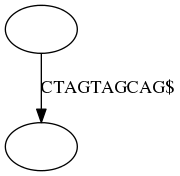
\includegraphics[width=0.15\textwidth]{tast1ai/tree_step01.png}
 }
 \subfigure[step 2]{
  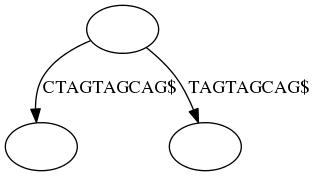
\includegraphics[width=0.25\textwidth]{tast1ai/tree_step02.png}
 }
 \subfigure[step 3]{
  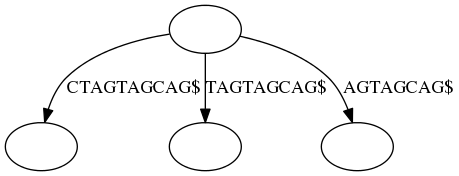
\includegraphics[width=0.35\textwidth]{tast1ai/tree_step03.png}
 }
 \subfigure[step 4]{
  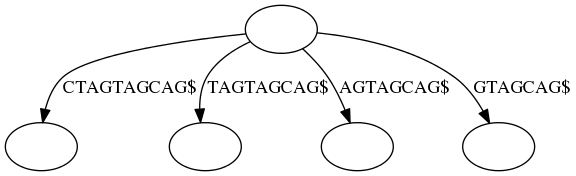
\includegraphics[width=0.45\textwidth]{tast1ai/tree_step04.png}
 }
 \subfigure[step 5]{
  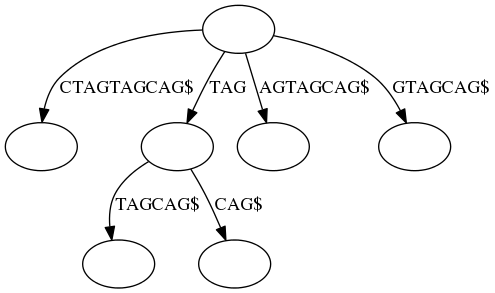
\includegraphics[width=0.45\textwidth]{tast1ai/tree_step05.png}
 }
 \subfigure[step 6]{
  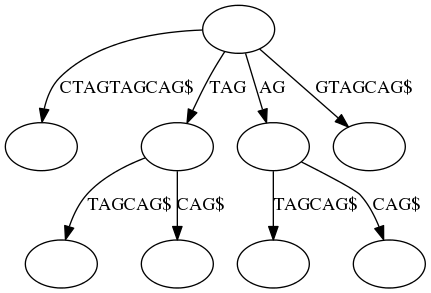
\includegraphics[width=0.45\textwidth]{tast1ai/tree_step06.png}
 }
 \subfigure[step 7]{
  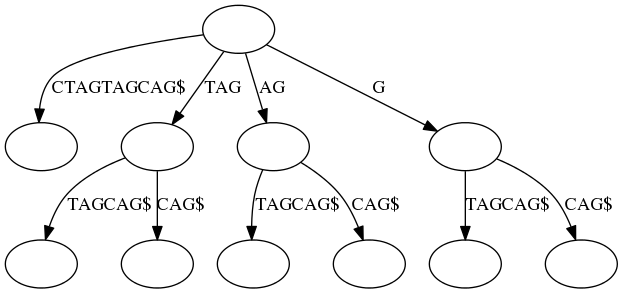
\includegraphics[width=0.45\textwidth]{tast1ai/tree_step07.png}
 }
 \subfigure[step 8]{
  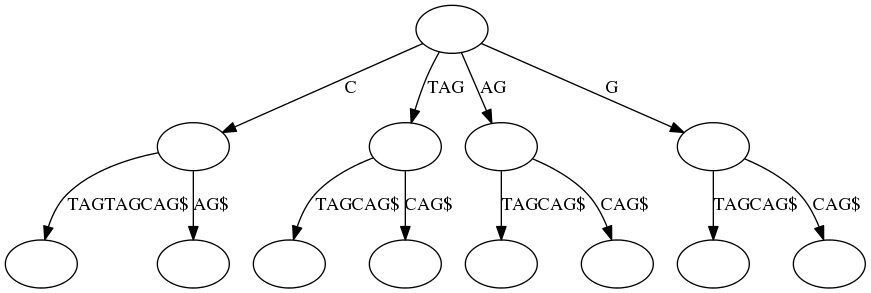
\includegraphics[width=0.45\textwidth]{tast1ai/tree_step08.png}
 }
 \subfigure[step 9]{
  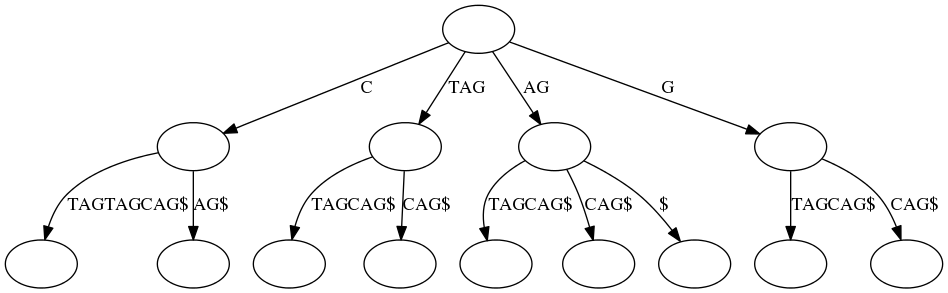
\includegraphics[width=0.45\textwidth]{tast1ai/tree_step09.png}
 }
 \subfigure[step 10]{
  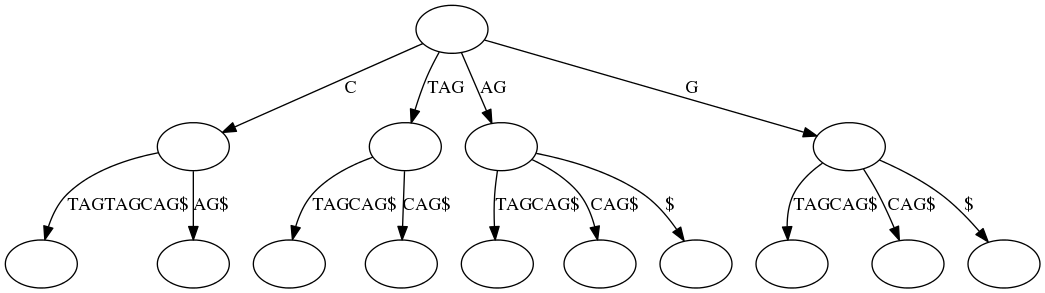
\includegraphics[width=0.7\textwidth]{tast1ai/tree_step10.png}
 }
 \subfigure[step 11]{
  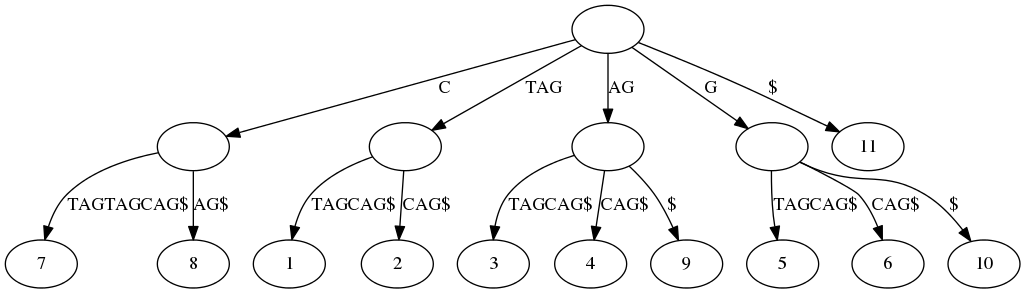
\includegraphics[width=0.7\textwidth]{tast1ai/tree_step11.png}
 }
 \caption{All steps of the naive implementation of suffix tree construction for the string ``CTAGTAGCAG''.}
 \label{fig:naiveImpl}
\end{figure}

\subsubsection*{ii}


\subsection*{b - \textit{Main data table of WOTD}}


\subsection*{c - \textit{Suffix tree application}}



\section*{Theoretical Assignment - \textit{Runtime and space complexity of suffix trees}}

\subsection*{a}
Assume a text $T$ of length $n$ with $n$ times the letter ``a''. If one build a suffix tree for $T$ 
using WOTD, each node will have just one c-group with all remaining suffixes in it. So evaluating the 
root node, one has to compute the longest common prefix of $n$ suffixes, of $n-1$ suffixes for the 
second node and so on. In each c-group the shortest suffix is of length $1$, so for each node $\overline{u}$ 
there are just $|R_a\{\overline{u}\}|$ numbers of comparisons.

Since $T$ is of length $n$ this will lead to an overall runtime of $\sum_{i=1}^{n}i = \frac{1}{2}n(n+1)$, 
which is in $O(n^2)$. $\square$


\subsection*{b}
Suffix links are defined as an auxiliary edge that point from branching node $\overline{bw}$ to the branching 
node $\overline{w}$, if it exists and to the root otherwise. If we now defined a suffix link, such that it 
points into the other direction (i.e. from branching node $\overline{w}$ to branching node $\overline{bw}$) gives 
us an efficient method to find maximal unique matches. If we now find a branching node that indicates 
a unique match (for definition see script) and there is a suffix link that point to another branching node, we know that the current 
branching node is not a maximal unique match (because it is not left maximal). So we just have to 
follow the suffix links until we reach a branching node without an outgoing suffix link and we have 
found a maximal unique match.


\subsection*{c}
A relevant suffix is defined as a suffix that leads to a modification of the tree topology, if it is 
inserted. 


\end{document}